% ============================================================
%  SESSION 6 — Next.js Giriş
%  XeLaTeX ile derleyin: xelatex session-06.tex
% ============================================================
\documentclass[12pt, a4paper]{article}

% ---------- Font & Dil ----------
\usepackage{fontspec}
\usepackage[turkish, shorthands=off]{babel}
\setmainfont{Georgia}
\setsansfont{Arial}
\setmonofont{Courier New}

% ---------- Sayfa Düzeni ----------
\usepackage[top=2.2cm, bottom=2.2cm, left=2.4cm, right=2.4cm]{geometry}
\usepackage{parskip}
\setlength{\parindent}{0pt}

% ---------- Renkler ----------
\usepackage{xcolor}
\definecolor{primary}{HTML}{2563EB}
\definecolor{secondary}{HTML}{7C3AED}
\definecolor{accent}{HTML}{059669}
\definecolor{warning}{HTML}{D97706}
\definecolor{danger}{HTML}{DC2626}
\definecolor{lightbg}{HTML}{F1F5F9}
\definecolor{codebg}{HTML}{1E293B}
\definecolor{codefg}{HTML}{E2E8F0}
\definecolor{reactblue}{HTML}{61DAFB}
\definecolor{jsxcol}{HTML}{93C5FD}
\definecolor{propscol}{HTML}{FCA5A5}
\definecolor{statecol}{HTML}{86EFAC}
\definecolor{jskw}{HTML}{93C5FD}
\definecolor{jsstr}{HTML}{86EFAC}
\definecolor{jscomment}{HTML}{94A3B8}
\definecolor{nextcol}{HTML}{000000}
\definecolor{ssrcol}{HTML}{8B5CF6}
\definecolor{csrcol}{HTML}{F59E0B}
\definecolor{routecol}{HTML}{EC4899}

% ---------- Kutular (tcolorbox) ----------
\usepackage[skins, breakable, listings]{tcolorbox}
\tcbuselibrary{skins, breakable, listings}

\newtcolorbox{infobox}[1][]{
  enhanced, breakable,
  colback=primary!8, colframe=primary,
  fonttitle=\bfseries\sffamily,
  title={#1},
  left=6pt, right=6pt, top=4pt, bottom=4pt,
  arc=4pt
}

\newtcolorbox{warningbox}[1][]{
  enhanced, breakable,
  colback=warning!10, colframe=warning,
  fonttitle=\bfseries\sffamily,
  title={#1},
  left=6pt, right=6pt, top=4pt, bottom=4pt,
  arc=4pt
}

\newtcolorbox{practicebox}[1][]{
  enhanced, breakable,
  colback=accent!8, colframe=accent,
  fonttitle=\bfseries\sffamily,
  title={#1},
  left=6pt, right=6pt, top=4pt, bottom=4pt,
  arc=4pt
}

\newtcolorbox{definebox}[1][]{
  enhanced, breakable,
  colback=secondary!7, colframe=secondary,
  fonttitle=\bfseries\sffamily,
  title={#1},
  left=6pt, right=6pt, top=4pt, bottom=4pt,
  arc=4pt
}

\newtcolorbox{dangerbox}[1][]{
  enhanced, breakable,
  colback=danger!7, colframe=danger,
  fonttitle=\bfseries\sffamily,
  title={#1},
  left=6pt, right=6pt, top=4pt, bottom=4pt,
  arc=4pt
}

% ---------- Kod Listeleme ----------
\usepackage{listings}

\lstset{literate=
  {ı}{{\texttt{i}}}1  {İ}{{\texttt{I}}}1
  {ğ}{{\texttt{g}}}1  {Ğ}{{\texttt{G}}}1
  {ş}{{\texttt{s}}}1  {Ş}{{\texttt{S}}}1
  {ü}{{\texttt{u}}}1  {Ü}{{\texttt{U}}}1
  {ö}{{\texttt{o}}}1  {Ö}{{\texttt{O}}}1
  {ç}{{\texttt{c}}}1  {Ç}{{\texttt{C}}}1
}

\lstdefinestyle{jsxstyle}{
  backgroundcolor=\color{codebg},
  basicstyle=\ttfamily\small\color{codefg},
  keywordstyle=\color{jskw}\bfseries,
  stringstyle=\color{jsstr},
  commentstyle=\color{jscomment}\itshape,
  morekeywords={let, const, var, async, await, of, from, import, export,
    default, class, extends, new, return, true, false, null, undefined,
    function, arrow, Promise, fetch, then, catch, finally, try,
    map, filter, reduce, forEach, find, findIndex, some, every,
    console, log, JSON, stringify, parse,
    React, useState, useEffect, useRef, useCallback, useMemo,
    props, children,
    onClick, onChange, onSubmit, onBlur, key, className, style, value,
    disabled, required, placeholder, type, htmlFor, checked,
    div, span, button, input, form, label, h1, h2, h3, p, ul, li, img,
    select, option, textarea, nav, a, main, header, footer,
    interface, type, Link, useRouter, usePathname, useParams,
    Metadata, Layout, Page, params, searchParams},
  morestring=[b]",
  morestring=[b]',
  morestring=[b]`,
  morecomment=[l]{//},
  morecomment=[s]{/*}{*/},
  showstringspaces=false,
  breaklines=true,
  frame=none,
  xleftmargin=8pt, xrightmargin=8pt,
}

\lstdefinestyle{shellstyle}{
  backgroundcolor=\color{codebg},
  basicstyle=\ttfamily\small\color{codefg},
  showstringspaces=false,
  breaklines=true,
  frame=none,
  xleftmargin=8pt, xrightmargin=8pt,
}

% ---------- Grafikler ----------
\usepackage{graphicx}
\usepackage{caption}
\usepackage{tikz}
\usetikzlibrary{arrows.meta, shapes.geometric, positioning, calc}

% ---------- Tablo ----------
\usepackage{booktabs}
\usepackage{tabularx}
\usepackage{array}

% ---------- Başlık Stilleri ----------
\makeatletter
\renewcommand{\section}{%
  \@startsection{section}{1}{\z@}%
    {-1.5ex plus -1ex minus -0.5ex}%
    {0.8ex plus 0.3ex}%
    {\normalfont\Large\bfseries\sffamily\color{primary}}%
}
\renewcommand{\subsection}{%
  \@startsection{subsection}{2}{\z@}%
    {-1.2ex plus -0.8ex minus -0.4ex}%
    {0.5ex plus 0.2ex}%
    {\normalfont\large\bfseries\sffamily\color{secondary}}%
}
\renewcommand{\subsubsection}{%
  \@startsection{subsubsection}{3}{\z@}%
    {-1ex plus -0.6ex minus -0.3ex}%
    {0.4ex}%
    {\normalfont\normalsize\bfseries\sffamily\color{accent}}%
}
\makeatother

% ---------- Üstbilgi / Altbilgi ----------
\usepackage{fancyhdr}
\setlength{\headheight}{14pt}
\pagestyle{fancy}
\fancyhf{}
\fancyhead[L]{\small\sffamily\color{gray} Front-end + Next.js Eğitimi}
\fancyhead[R]{\small\sffamily\color{gray} Session 6 --- Next.js Giriş}
\fancyfoot[C]{\small\sffamily\color{gray} \thepage}
\renewcommand{\headrulewidth}{0.4pt}

% ---------- Diğer ----------
\usepackage{enumitem}
\setlist[itemize]{leftmargin=1.5em, itemsep=2pt}
\setlist[enumerate]{leftmargin=1.5em, itemsep=2pt}
\usepackage{hyperref}
\hypersetup{colorlinks=true, linkcolor=primary, urlcolor=primary}
\usepackage{fontawesome5}

% ---------- Yardımcı Komut ----------
\newcommand{\timebadge}[1]{%
  \noindent
  \colorbox{primary}{\color{white}\sffamily\bfseries\small\strut~~\faStopwatch~~#1~~}%
  \par\vspace{4pt}%
}

\newcommand{\jsinline}[1]{\texttt{\color{primary}#1}}

% ============================================================
\begin{document}

% ============================================================
%  KAPAK
% ============================================================
\thispagestyle{empty}

\begin{tikzpicture}[remember picture, overlay]
  \fill[primary] (current page.north west)
    rectangle ++(\paperwidth, -8.0cm);
  \fill[secondary] (current page.north west) ++(0,-7.8cm)
    rectangle ++(\paperwidth, -0.28cm);
\end{tikzpicture}

\vspace*{1.6cm}
{\color{white}\sffamily
  \hspace{1.2cm}{\small SESSION 6 / 8 \quad|\quad 11 Mayıs 2026 \quad|\quad~90 dakika}\\[12pt]
  \hspace{1.2cm}{\fontsize{30}{36}\selectfont\bfseries Next.js Giriş}\\[8pt]
  \hspace{1.2cm}{\Large SSR/CSR, Routing, Layout ve Sayfa Yapısı}
}

\vspace{0.9cm}

\vspace{0.1cm}

\begin{tcolorbox}[enhanced,
  colback=lightbg, colframe=gray!30, arc=4pt,
  title={\sffamily\bfseries\color{primary}\faStream\quad Session Akışı},
  fonttitle=\bfseries\sffamily]
\sffamily\small
\begin{tabularx}{\textwidth}{>{\bfseries\color{primary}}l X l}
\toprule
Süre & Konu & Anahtar Kavramlar \\
\midrule
0--20 dk  & Next.js Nedir, Neden Var?           & SSR vs CSR, framework vs library \\
20--50 dk & File-Based Routing                  & app/ klasörü, Link, dinamik route \\
50--70 dk & Layout ve Sayfa Organizasyonu       & layout.tsx, nested layouts \\
70--90 dk & \textcolor{accent}{Pratik: Liste + Detay} & dinamik route, params \\
\bottomrule
\end{tabularx}
\end{tcolorbox}

% ============================================================
\clearpage
\section{\faRocket\ Next.js Nedir, Neden Var?}
\timebadge{0--20 dakika}

\subsection{React'tan Sonra Ne Eksik Kalıyor?}

Şu ana kadar React ile arayüz geliştirmeyi öğrendik. Ama gerçek bir
uygulamada React tek başına yeterli değil:

\begin{itemize}
  \item \textbf{Routing} --- birden fazla sayfa nasıl yönetilir?
  \item \textbf{SEO} --- arama motorları sayfanızı nasıl indeksler?
  \item \textbf{İlk yükleme hızı} --- boş HTML + büyük JS dosyası yavaş açılır
  \item \textbf{Sunucu tarafı veri çekme} --- API key'leri client'ta göstermek istemeyiz
  \item \textbf{Image optimization, fonts, caching\ldots}
\end{itemize}

\vspace{6pt}

\begin{definebox}[Next.js Nedir?]
Next.js, Vercel tarafından geliştirilen, \textbf{React üzerine kurulmuş
bir framework}'tür. React'ın eksik bıraktığı kısımları (routing, SSR,
optimizasyon, build sistemi\ldots) hazır olarak sunar.

\vspace{4pt}
\textbf{Library vs Framework:} React bir kütüphanedir (siz çağırırsınız).
Next.js bir framework'tür (o sizi çağırır --- dosya yapısı, kuralları belli).
\end{definebox}

\vspace{6pt}

\begin{infobox}[\faInfoCircle\ Şirkette Neden Next.js?]
\begin{itemize}
  \item Kurumsal projelerde \textbf{SEO} ve \textbf{performans} kritik
  \item File-based routing ile takım içinde tutarlı yapı
  \item Built-in optimizasyonlar (image, font, code-splitting)
  \item TypeScript, ESLint, CSS desteği out-of-the-box
  \item Vercel, AWS, kendi sunucumuz --- her yere deploy edilebilir
\end{itemize}
\end{infobox}

% ----------------------------------------------------------
\subsection{Rendering Stratejileri --- CSR vs SSR}

\subsubsection{CSR --- Client-Side Rendering}

Saf React (Vite, CRA) bu şekilde çalışır:

\vspace{6pt}

\begin{center}
\begin{tikzpicture}[node distance=0.5cm, >=Stealth, font=\sffamily\footnotesize]

  \node[font=\sffamily\bfseries\small, text=csrcol] at (0, 4.6) {CSR (Client-Side Rendering):};

  % Boş HTML
  \fill[danger!20] (0.0,3.4) rectangle (2.2,4.1);
  \node at (1.1, 3.75) {1. Boş HTML};
  \draw[->, thick, gray!50] (2.2,3.75) -- (2.4,3.75);

  % JS indir
  \fill[warning!30] (2.4,3.4) rectangle (4.8,4.1);
  \node at (3.6, 3.75) {2. Büyük JS indir};
  \draw[->, thick, gray!50] (4.8,3.75) -- (5.0,3.75);

  % JS çalışır
  \fill[warning!30] (5.0,3.4) rectangle (7.4,4.1);
  \node at (6.2, 3.75) {3. JS çalışır};
  \draw[->, thick, gray!50] (7.4,3.75) -- (7.6,3.75);

  % API
  \fill[warning!30] (7.6,3.4) rectangle (10.0,4.1);
  \node at (8.8, 3.75) {4. API'den veri};
  \draw[->, thick, gray!50] (10.0,3.75) -- (10.2,3.75);

  % Render
  \fill[accent!30] (10.2,3.4) rectangle (12.0,4.1);
  \node at (11.1, 3.75) {5. Ekran};

  \node[font=\sffamily\tiny\color{danger}, below] at (6.0, 3.35)
    {Kullanıcı bu süre boyunca beyaz ekran görür};

  % Pros / Cons
  \node[font=\sffamily\bfseries\small, accent] at (1.6, 2.4) {\faCheck\ Artılar:};
  \node[font=\sffamily\small, anchor=west] at (0, 1.9) {Sayfa geçişleri hızlı};
  \node[font=\sffamily\small, anchor=west] at (0, 1.5) {Sunucu yükü az};
  \node[font=\sffamily\small, anchor=west] at (0, 1.1) {Basit deploy};

  \node[font=\sffamily\bfseries\small, danger] at (8.0, 2.4) {\faTimes\ Eksiler:};
  \node[font=\sffamily\small, anchor=west] at (6.5, 1.9) {İlk yükleme yavaş};
  \node[font=\sffamily\small, anchor=west] at (6.5, 1.5) {SEO zayıf (bot boş HTML görür)};
  \node[font=\sffamily\small, anchor=west] at (6.5, 1.1) {Yavaş cihazda JS yavaş çalışır};

\end{tikzpicture}
\end{center}

\vspace{6pt}

\subsubsection{SSR --- Server-Side Rendering}

Next.js varsayılan olarak sayfaları sunucuda render eder:

\vspace{6pt}

\begin{center}
\begin{tikzpicture}[node distance=0.5cm, >=Stealth, font=\sffamily\footnotesize]

  \node[font=\sffamily\bfseries\small, text=ssrcol] at (0, 4.6) {SSR (Server-Side Rendering):};

  % Server render
  \fill[ssrcol!30] (0.0,3.4) rectangle (3.0,4.1);
  \node at (1.5, 3.75) {1. Sunucuda render};
  \draw[->, thick, gray!50] (3.0,3.75) -- (3.2,3.75);

  % Hazır HTML
  \fill[accent!30] (3.2,3.4) rectangle (6.4,4.1);
  \node at (4.8, 3.75) {2. Hazır HTML gelir};
  \draw[->, thick, gray!50] (6.4,3.75) -- (6.6,3.75);

  % Ekran
  \fill[accent!30] (6.6,3.4) rectangle (8.6,4.1);
  \node at (7.6, 3.75) {3. İçerik görünür};
  \draw[->, thick, gray!50] (8.6,3.75) -- (8.8,3.75);

  % JS hydrate
  \fill[primary!30] (8.8,3.4) rectangle (12.0,4.1);
  \node at (10.4, 3.75) {4. JS yüklenir (hydrate)};

  \node[font=\sffamily\tiny\color{accent}, below] at (6.0, 3.35)
    {Kullanıcı içeriği çok hızlı görür};

  % Pros / Cons
  \node[font=\sffamily\bfseries\small, accent] at (1.6, 2.4) {\faCheck\ Artılar:};
  \node[font=\sffamily\small, anchor=west] at (0, 1.9) {SEO mükemmel};
  \node[font=\sffamily\small, anchor=west] at (0, 1.5) {İlk yükleme hızlı};
  \node[font=\sffamily\small, anchor=west] at (0, 1.1) {Yavaş cihazda sorun yok};

  \node[font=\sffamily\bfseries\small, danger] at (8.0, 2.4) {\faTimes\ Eksiler:};
  \node[font=\sffamily\small, anchor=west] at (6.5, 1.9) {Sunucu gerekli};
  \node[font=\sffamily\small, anchor=west] at (6.5, 1.5) {Her istek sunucuyu yorar};
  \node[font=\sffamily\small, anchor=west] at (6.5, 1.1) {Biraz daha karmaşık};

\end{tikzpicture}
\end{center}

\vspace{6pt}

\begin{infobox}[\faLightbulb\ Basit Bir Analoji]
\textbf{CSR:} Restorana gider, masaya boş bir tabak konur, kendi yemeğinizi
yaparsınız.\\
\textbf{SSR:} Yemek mutfakta hazırlanır, sıcak sıcak masaya gelir.
\end{infobox}

% ----------------------------------------------------------
\newpage
\subsection{Karşılaştırma Tablosu}

\begin{tcolorbox}[enhanced, colback=lightbg, colframe=gray!30, arc=4pt]
\sffamily\small
\begin{tabularx}{\textwidth}{>{\bfseries\color{primary}}l X X}
\toprule
Özellik & CSR (saf React) & SSR (Next.js) \\
\midrule
İlk yükleme        & Yavaş --- beyaz ekran  & Hızlı --- hazır HTML \\[4pt]
SEO                & Zayıf                  & Güçlü \\[4pt]
Sayfa geçişleri    & Hızlı                  & Hızlı (client-side nav) \\[4pt]
Sunucu yükü        & Düşük                  & Yüksek \\[4pt]
Veri çekme         & Browser'dan API'ye     & Sunucudan API'ye \\[4pt]
API key güvenliği  & Sızabilir              & Sunucuda kalır \\[4pt]
Karmaşıklık        & Düşük                  & Orta \\
\bottomrule
\end{tabularx}
\end{tcolorbox}

\vspace{6pt}

\begin{warningbox}[\faExclamationTriangle\ Next.js Sadece SSR mı?]
Hayır. Next.js, sayfa başına strateji seçmenize izin verir:
\begin{itemize}
  \item \textbf{SSR} --- her istekte sunucuda render
  \item \textbf{SSG} --- build zamanında bir kere render (blog, landing page)
  \item \textbf{CSR} --- belirli component'leri client'ta render (\texttt{"use client"})
  \item \textbf{ISR} --- belirli aralıkla yeniden render
\end{itemize}
Şimdilik varsayılan davranışla (Server Components) çalışacağız.
\end{warningbox}

% ============================================================
\newpage
\section{\faFolder\ File-Based Routing}
\timebadge{20--50 dakika}

\subsection{Proje Kurulumu}

\begin{tcolorbox}[enhanced, colback=codebg, colframe=gray!30,
    colbacktitle=primary!85!black, coltitle=white, arc=4pt,
    title={\sffamily\bfseries\small Next.js Projesi Oluşturma}]
\begin{lstlisting}[style=shellstyle]
npx create-next-app@latest my-app

# Sorulan secenekler:
# TypeScript?   Yes
# ESLint?       Yes
# Tailwind CSS? Yes (veya No --- bizim icin opsiyonel)
# src/ dir?     Yes (onerilen)
# App Router?   Yes (modern yaklasim)
# Turbopack?    Yes (hizli)

cd my-app
npm run dev
# http://localhost:3000
\end{lstlisting}
\end{tcolorbox}

\vspace{6pt}

\subsection{App Router --- Klasör = Route}

\begin{definebox}[File-Based Routing]
Next.js'te \textbf{her klasör bir URL segment'idir} ve içindeki
\texttt{page.tsx} dosyası o URL'in sayfasını oluşturur. Manuel route
tanımı yoktur --- dosya yapısı URL yapısıdır.
\end{definebox}

\vspace{6pt}

\begin{center}
\begin{tikzpicture}[font=\ttfamily\small]
  \node[anchor=west, primary] at (0,    3.6) {src/};
  \node[anchor=west]          at (0.5,  3.0) {└── app/};
  \node[anchor=west, secondary] at (1.0,  2.4) {├── layout.tsx};
  \node[anchor=west, gray]    at (4.5,  2.4) {\footnotesize $\rightarrow$ tüm sayfaların kabuğu};
  \node[anchor=west, secondary] at (1.0,  1.8) {├── page.tsx};
  \node[anchor=west, gray]    at (4.5,  1.8) {\footnotesize $\rightarrow$ /};
  \node[anchor=west, primary] at (1.0,  1.2) {├── about/};
  \node[anchor=west, secondary] at (1.6,  0.6) {│   └── page.tsx};
  \node[anchor=west, gray]    at (4.5,  0.6) {\footnotesize $\rightarrow$ /about};
  \node[anchor=west, primary] at (1.0,  0.0) {├── blog/};
  \node[anchor=west, secondary] at (1.6, -0.6) {│   ├── page.tsx};
  \node[anchor=west, gray]    at (4.5, -0.6) {\footnotesize $\rightarrow$ /blog};
  \node[anchor=west, primary] at (1.6, -1.2) {│   └── [slug]/};
  \node[anchor=west, secondary] at (2.2, -1.8) {│       └── page.tsx};
  \node[anchor=west, gray]    at (4.5, -1.8) {\footnotesize $\rightarrow$ /blog/herhangi-bir-yazi};
\end{tikzpicture}
\end{center}

\vspace{8pt}

\begin{tcolorbox}[enhanced, colback=lightbg, colframe=gray!30, arc=4pt]
\sffamily\small
\begin{tabularx}{\textwidth}{>{\ttfamily\color{primary}}l X}
\toprule
\normalfont\bfseries Dosya / Klasör & \normalfont\bfseries Anlamı \\
\midrule
page.tsx       & O route'un sayfası (UI) \\
layout.tsx     & O route ve altındaki tüm sayfaların ortak çerçevesi \\
loading.tsx    & Yüklenme sırasında gösterilecek UI \\
error.tsx      & Hata olduğunda gösterilecek UI \\
not-found.tsx  & 404 sayfası \\
{[slug]}       & Dinamik segment --- URL'den parametre alır \\
(group)        & Klasörü route'a katmaz, sadece organizasyon için \\
\bottomrule
\end{tabularx}
\end{tcolorbox}

% ----------------------------------------------------------
\newpage
\subsection{İlk Sayfa --- page.tsx}

\begin{tcolorbox}[enhanced, colback=codebg, colframe=gray!30,
    colbacktitle=primary!85!black, coltitle=white, arc=4pt,
    title={\sffamily\bfseries\small src/app/page.tsx (anasayfa)}]
\begin{lstlisting}[style=jsxstyle]
export default function HomePage() {
  return (
    <main>
      <h1>Anasayfa</h1>
      <p>Hosgeldin!</p>
    </main>
  );
}
\end{lstlisting}
\end{tcolorbox}

\vspace{6pt}

\begin{tcolorbox}[enhanced, colback=codebg, colframe=gray!30,
    colbacktitle=primary!85!black, coltitle=white, arc=4pt,
    title={\sffamily\bfseries\small src/app/about/page.tsx (/about)}]
\begin{lstlisting}[style=jsxstyle]
export default function AboutPage() {
  return (
    <main>
      <h1>Hakkimizda</h1>
      <p>Biz kimiz, ne yapariz...</p>
    </main>
  );
}
\end{lstlisting}
\end{tcolorbox}

\vspace{6pt}

\begin{infobox}[\faLightbulb\ Önemli Nokta]
Page component'i \textbf{default export} olmalıdır. İsmi ne olursa olsun
(\texttt{HomePage}, \texttt{Page}, \texttt{X}) Next.js \texttt{export default}'u
kullanır.
\end{infobox}

% ----------------------------------------------------------
\subsection{Sayfalar Arası Geçiş --- Link Component}

HTML'deki \texttt{<a href="">} kullanmak \textbf{tüm sayfayı yeniden yükler}.
SPA hissini koruyabilmek için Next.js'in \texttt{<Link>} component'ini kullanırız.

\vspace{6pt}

\begin{tcolorbox}[enhanced, colback=codebg, colframe=gray!30,
    colbacktitle=primary!85!black, coltitle=white, arc=4pt,
    title={\sffamily\bfseries\small Link Kullanımı}]
\begin{lstlisting}[style=jsxstyle]
import Link from "next/link";

export default function Navbar() {
  return (
    <nav>
      <Link href="/">Anasayfa</Link>
      <Link href="/about">Hakkimizda</Link>
      <Link href="/blog">Blog</Link>
      <Link href="/blog/ilk-yazi">Ilk Yazi</Link>
    </nav>
  );
}
\end{lstlisting}
\end{tcolorbox}

\vspace{6pt}

\begin{tcolorbox}[enhanced, colback=lightbg, colframe=gray!30, arc=4pt]
\sffamily\small
\begin{tabularx}{\textwidth}{X X}
\toprule
\bfseries \texttt{<a href="">} & \bfseries \texttt{<Link href="">} \\
\midrule
Tüm sayfa yeniden yüklenir & Sadece içerik değişir (client-side nav) \\
JS state sıfırlanır & State korunur \\
Yavaş --- sayfa flash eder & Hızlı --- akıcı geçiş \\
Hedef sayfa prefetch edilmez & Hedef sayfa arka planda prefetch edilir \\
\bottomrule
\end{tabularx}
\end{tcolorbox}

\vspace{6pt}

\begin{warningbox}[\faExclamationTriangle\ Dikkat]
\texttt{<Link>} \textbf{sadece uygulama içi} linkler için kullanılır.
Dış sayfalara (\texttt{https://google.com}) link verirken normal
\texttt{<a>} kullanın.
\end{warningbox}

% ----------------------------------------------------------
\newpage
\subsection{Dinamik Route'lar --- {[slug]} Klasörü}

URL'in bir kısmının değişken olması gerektiğinde köşeli parantezli
klasör kullanılır:

\vspace{6pt}

\begin{tcolorbox}[enhanced, colback=lightbg, colframe=gray!30, arc=4pt]
\sffamily\small
\begin{tabularx}{\textwidth}{>{\ttfamily\color{primary}}l X}
\toprule
\normalfont\bfseries Klasör & \normalfont\bfseries Eşleşen URL'ler \\
\midrule
blog/[slug]/page.tsx    & /blog/hello, /blog/abc, /blog/123 \\
products/[id]/page.tsx  & /products/1, /products/42 \\
users/[userId]/page.tsx & /users/ali, /users/zeynep \\
\bottomrule
\end{tabularx}
\end{tcolorbox}

\vspace{6pt}

\begin{tcolorbox}[enhanced, colback=codebg, colframe=gray!30,
    colbacktitle=routecol!85!black, coltitle=white, arc=4pt,
    title={\sffamily\bfseries\small src/app/blog/[slug]/page.tsx}]
\begin{lstlisting}[style=jsxstyle]
interface Props {
  params: Promise<{ slug: string }>;
}

export default async function BlogPostPage({ params }: Props) {
  const { slug } = await params;

  return (
    <main>
      <h1>Yazi: {slug}</h1>
      <p>URL'den gelen slug: <strong>{slug}</strong></p>
    </main>
  );
}
\end{lstlisting}
\end{tcolorbox}

\vspace{6pt}

\begin{infobox}[\faLightbulb\ Neden async ve await?]
Next.js'in son sürümlerinde \texttt{params} bir Promise'dir.
Component'i \texttt{async} yaparak \texttt{await params} ile değeri alırız.
Server component'ler async olabilir --- bu React'tan farklı bir özelliktir!
\end{infobox}

\vspace{6pt}

\subsubsection{Çoklu Dinamik Segment}

\begin{tcolorbox}[enhanced, colback=codebg, colframe=gray!30,
    colbacktitle=routecol!85!black, coltitle=white, arc=4pt,
    title={\sffamily\bfseries\small src/app/users/[userId]/posts/[postId]/page.tsx}]
\begin{lstlisting}[style=jsxstyle]
interface Props {
  params: Promise<{ userId: string; postId: string }>;
}

export default async function UserPostPage({ params }: Props) {
  const { userId, postId } = await params;
  // /users/ali/posts/3 --> userId="ali", postId="3"

  return (
    <main>
      <p>Kullanici: {userId}</p>
      <p>Post: {postId}</p>
    </main>
  );
}
\end{lstlisting}
\end{tcolorbox}

\vspace{6pt}

\subsection{Sayfada Veri Çekme}

Server component'ler doğrudan \texttt{async} olabildiği için, veri çekme
çok basitleşir:

\vspace{6pt}

\begin{tcolorbox}[enhanced, colback=codebg, colframe=gray!30,
    colbacktitle=ssrcol!85!black, coltitle=white, arc=4pt,
    title={\sffamily\bfseries\small Sunucu Tarafında Veri Çekme}]
\begin{lstlisting}[style=jsxstyle]
// src/app/blog/page.tsx
interface Post {
  id: number;
  title: string;
  body: string;
}

export default async function BlogPage() {
  // Bu kod SUNUCUDA calisir --- browser'a hic gelmez!
  const res = await fetch(
    "https://jsonplaceholder.typicode.com/posts?_limit=10"
  );
  const posts: Post[] = await res.json();

  return (
    <main>
      <h1>Blog</h1>
      <ul>
        {posts.map(p => (
          <li key={p.id}>{p.title}</li>
        ))}
      </ul>
    </main>
  );
}
\end{lstlisting}
\end{tcolorbox}

\vspace{6pt}

\begin{infobox}[\faMagic\ Bu Ne Anlama Geliyor?]
\begin{itemize}
  \item \texttt{useEffect} + \texttt{useState} + loading yönetimi \textbf{yok}
  \item \texttt{fetch} doğrudan component içinde \texttt{await} ile
  \item Veri sunucuda çekilir, kullanıcıya hazır HTML olarak gelir
  \item Tarayıcı network sekmesinde fetch görmezsiniz!
\end{itemize}
\end{infobox}

% ============================================================
\newpage
\section{\faLayerGroup\ Layout ve Sayfa Organizasyonu}
\timebadge{50--70 dakika}

\subsection{layout.tsx --- Ortak Kabuk}

\begin{definebox}[Layout Nedir?]
Layout, \textbf{birden fazla sayfanın paylaştığı UI çerçevesidir} ---
navbar, footer, sidebar gibi her sayfada görünecek parçalar.
\texttt{layout.tsx} \textbf{aynı klasördeki} \texttt{page.tsx} ve
\textbf{tüm alt klasörlerdeki} sayfaları sarar.
\end{definebox}

\vspace{6pt}

\subsubsection{Root Layout (Zorunlu)}

\begin{tcolorbox}[enhanced, colback=codebg, colframe=gray!30,
    colbacktitle=primary!85!black, coltitle=white, arc=4pt,
    title={\sffamily\bfseries\small src/app/layout.tsx}]
\begin{lstlisting}[style=jsxstyle]
import "./globals.css";
import Link from "next/link";

export const metadata = {
  title: "My App",
  description: "Next.js egitimi",
};

export default function RootLayout({
  children,
}: {
  children: React.ReactNode;
}) {
  return (
    <html lang="tr">
      <body>
        <header style={{ padding: 16, background: "#2563eb", color: "white" }}>
          <nav style={{ display: "flex", gap: 16 }}>
            <Link href="/" style={{ color: "white" }}>Anasayfa</Link>
            <Link href="/blog" style={{ color: "white" }}>Blog</Link>
            <Link href="/about" style={{ color: "white" }}>Hakkimizda</Link>
          </nav>
        </header>

        <main style={{ padding: 24 }}>
          {children} {/* Sayfa icerigi buraya gelir */}
        </main>

        <footer style={{ padding: 16, textAlign: "center", color: "#94a3b8" }}>
          <p>2026 Sirket Adi</p>
        </footer>
      </body>
    </html>
  );
}
\end{lstlisting}
\end{tcolorbox}

\vspace{6pt}

\begin{warningbox}[\faExclamationTriangle\ Root Layout Zorunluluğu]
\texttt{src/app/layout.tsx} \textbf{zorunludur} ve mutlaka
\texttt{<html>} + \texttt{<body>} etiketlerini içermelidir.
Diğer layout'lar opsiyoneldir ve bu etiketleri içermez.
\end{warningbox}

% ----------------------------------------------------------
\newpage
\subsection{Nested Layouts --- İç İçe Çerçeveler}

Alt klasörlere de \texttt{layout.tsx} koyabiliriz. Bu, root layout'un
\textbf{içinde} render olur. Örneğin sadece dashboard sayfalarında
sidebar göstermek istiyorsak:

\vspace{6pt}

\begin{center}
\begin{tikzpicture}[font=\ttfamily\small]
  \node[anchor=west, primary] at (0,   3.6) {src/app/};
  \node[anchor=west, secondary] at (0.5, 3.0) {├── layout.tsx};
  \node[anchor=west, gray]    at (3.5, 3.0) {\footnotesize (root: header + footer)};
  \node[anchor=west, secondary] at (0.5, 2.4) {├── page.tsx};
  \node[anchor=west, primary] at (0.5, 1.8) {└── dashboard/};
  \node[anchor=west, secondary] at (1.0, 1.2) {├── layout.tsx};
  \node[anchor=west, gray]    at (3.5, 1.2) {\footnotesize (dashboard: + sidebar)};
  \node[anchor=west, secondary] at (1.0, 0.6) {├── page.tsx};
  \node[anchor=west, primary] at (1.0, 0.0) {├── settings/};
  \node[anchor=west, secondary] at (1.5,-0.6) {│   └── page.tsx};
  \node[anchor=west, primary] at (1.0,-1.2) {└── profile/};
  \node[anchor=west, secondary] at (1.5,-1.8) {\quad\quad└── page.tsx};
\end{tikzpicture}
\end{center}

\vspace{6pt}

\begin{tcolorbox}[enhanced, colback=codebg, colframe=gray!30,
    colbacktitle=primary!85!black, coltitle=white, arc=4pt,
    title={\sffamily\bfseries\small src/app/dashboard/layout.tsx}]
\begin{lstlisting}[style=jsxstyle]
import Link from "next/link";

export default function DashboardLayout({
  children,
}: {
  children: React.ReactNode;
}) {
  return (
    <div style={{ display: "flex", gap: 24 }}>
      <aside style={{ width: 200 }}>
        <h3>Dashboard</h3>
        <nav style={{ display: "flex", flexDirection: "column", gap: 8 }}>
          <Link href="/dashboard">Anasayfa</Link>
          <Link href="/dashboard/settings">Ayarlar</Link>
          <Link href="/dashboard/profile">Profil</Link>
        </nav>
      </aside>

      <section style={{ flex: 1 }}>
        {children}
      </section>
    </div>
  );
}
\end{lstlisting}
\end{tcolorbox}

\vspace{6pt}

\begin{infobox}[\faSitemap\ İç İçe Render Sırası]
\texttt{/dashboard/settings} URL'i şu şekilde render olur:

\vspace{4pt}
\texttt{RootLayout} (header + footer) $\rightarrow$
\texttt{DashboardLayout} (sidebar) $\rightarrow$
\texttt{SettingsPage}

\vspace{4pt}
Layout'lar iç içe geçer; her seviye \texttt{\{children\}} olarak bir
sonrakini render eder.
\end{infobox}

% ----------------------------------------------------------
\subsection{Metadata --- SEO için Önemli}

Her sayfanın veya layout'un kendi metadata'sı olabilir. Bu, sayfa
\texttt{<head>}'ine title, description gibi bilgiler ekler.

\vspace{6pt}

\begin{tcolorbox}[enhanced, colback=codebg, colframe=gray!30,
    colbacktitle=accent!85!black, coltitle=white, arc=4pt,
    title={\sffamily\bfseries\small Statik Metadata}]
\begin{lstlisting}[style=jsxstyle]
// src/app/about/page.tsx
import type { Metadata } from "next";

export const metadata: Metadata = {
  title: "Hakkimizda - My App",
  description: "Sirketimiz hakkinda bilgiler",
};

export default function AboutPage() {
  return <h1>Hakkimizda</h1>;
}
\end{lstlisting}
\end{tcolorbox}

\vspace{6pt}

\begin{tcolorbox}[enhanced, colback=codebg, colframe=gray!30,
    colbacktitle=accent!85!black, coltitle=white, arc=4pt,
    title={\sffamily\bfseries\small Dinamik Metadata --- URL'e Göre}]
\begin{lstlisting}[style=jsxstyle]
// src/app/blog/[slug]/page.tsx
import type { Metadata } from "next";

interface Props {
  params: Promise<{ slug: string }>;
}

export async function generateMetadata({ params }: Props): Promise<Metadata> {
  const { slug } = await params;

  return {
    title: `${slug} - Blog`,
    description: `${slug} yazisi`,
  };
}
\end{lstlisting}
\end{tcolorbox}

% ----------------------------------------------------------
\newpage
\subsection{Özel Dosyalar --- loading.tsx ve not-found.tsx}

\begin{tcolorbox}[enhanced, colback=codebg, colframe=gray!30,
    colbacktitle=warning!85!black, coltitle=white, arc=4pt,
    title={\sffamily\bfseries\small src/app/blog/loading.tsx}]
\begin{lstlisting}[style=jsxstyle]
// Bu sayfanin verisi yuklenirken otomatik gosterilir
export default function Loading() {
  return (
    <div style={{ padding: 40, textAlign: "center" }}>
      <p>Blog yazilari yukleniyor...</p>
    </div>
  );
}
\end{lstlisting}
\end{tcolorbox}

\vspace{6pt}

\begin{tcolorbox}[enhanced, colback=codebg, colframe=gray!30,
    colbacktitle=danger!85!black, coltitle=white, arc=4pt,
    title={\sffamily\bfseries\small src/app/not-found.tsx}]
\begin{lstlisting}[style=jsxstyle]
import Link from "next/link";

export default function NotFound() {
  return (
    <div style={{ padding: 40, textAlign: "center" }}>
      <h1>404 - Sayfa Bulunamadi</h1>
      <p>Aradiginiz sayfa mevcut degil.</p>
      <Link href="/">Anasayfaya don</Link>
    </div>
  );
}
\end{lstlisting}
\end{tcolorbox}

\vspace{6pt}

\begin{infobox}[\faLightbulb\ Özet --- Özel Dosyalar]
\begin{itemize}
  \item \texttt{page.tsx} --- sayfa içeriği
  \item \texttt{layout.tsx} --- ortak kabuk
  \item \texttt{loading.tsx} --- yüklenme göstergesi
  \item \texttt{error.tsx} --- hata yakalama (Session 7'de detay)
  \item \texttt{not-found.tsx} --- 404 sayfası
\end{itemize}
\end{infobox}

% ============================================================
\newpage
\section{\faHammer\ Pratik: Blog Listesi ve Detay Sayfası}
\timebadge{70--90 dakika}

\begin{practicebox}[\faTasks\ Pratik Hedef]
JSONPlaceholder API'sini kullanarak basit bir blog uygulaması yapalım:
\begin{enumerate}
  \item \texttt{/} --- Anasayfa
  \item \texttt{/blog} --- Tüm post'ların listesi (sunucu tarafında çekilir)
  \item \texttt{/blog/[id]} --- Bir post'un detayı (dinamik route)
  \item Tüm sayfalar için root layout (navbar)
  \item 404 sayfası
\end{enumerate}
\end{practicebox}

\vspace{8pt}

\subsection{Dosya Yapısı}

\begin{center}
\begin{tikzpicture}[font=\ttfamily\small]
  \node[anchor=west, primary] at (0,   2.4) {src/app/};
  \node[anchor=west, secondary] at (0.5, 1.8) {├── layout.tsx};
  \node[anchor=west, secondary] at (0.5, 1.2) {├── page.tsx};
  \node[anchor=west, secondary] at (0.5, 0.6) {├── not-found.tsx};
  \node[anchor=west, primary] at (0.5, 0.0) {└── blog/};
  \node[anchor=west, secondary] at (1.0,-0.6) {├── page.tsx};
  \node[anchor=west, secondary] at (1.0,-1.2) {├── loading.tsx};
  \node[anchor=west, primary] at (1.0,-1.8) {└── [id]/};
  \node[anchor=west, secondary] at (1.5,-2.4) {\quad\quad└── page.tsx};
\end{tikzpicture}
\end{center}

\vspace{8pt}

\subsection{Adım 1 --- Root Layout}

\begin{tcolorbox}[enhanced, colback=codebg, colframe=gray!30,
    colbacktitle=primary!85!black, coltitle=white, arc=4pt,
    title={\sffamily\bfseries\small src/app/layout.tsx}]
\begin{lstlisting}[style=jsxstyle]
import Link from "next/link";
import "./globals.css";

export const metadata = {
  title: "Mini Blog",
  description: "Next.js ile blog uygulamasi",
};

export default function RootLayout({
  children,
}: {
  children: React.ReactNode;
}) {
  return (
    <html lang="tr">
      <body>
        <header style={{ background: "#2563eb", padding: 16 }}>
          <nav style={{ display: "flex", gap: 16 }}>
            <Link href="/" style={{ color: "white" }}>Anasayfa</Link>
            <Link href="/blog" style={{ color: "white" }}>Blog</Link>
          </nav>
        </header>

        <main style={{ padding: 24, maxWidth: 800, margin: "0 auto" }}>
          {children}
        </main>
      </body>
    </html>
  );
}
\end{lstlisting}
\end{tcolorbox}

\subsection{Adım 2 --- Anasayfa}

\begin{tcolorbox}[enhanced, colback=codebg, colframe=gray!30,
    colbacktitle=primary!85!black, coltitle=white, arc=4pt,
    title={\sffamily\bfseries\small src/app/page.tsx}]
\begin{lstlisting}[style=jsxstyle]
import Link from "next/link";

export default function HomePage() {
  return (
    <div>
      <h1>Hosgeldin!</h1>
      <p>Bu Next.js ile yapilmis basit bir blog uygulamasidir.</p>
      <Link href="/blog">Yazilara goz at</Link>
    </div>
  );
}
\end{lstlisting}
\end{tcolorbox}

% ----------------------------------------------------------
\newpage
\subsection{Adım 3 --- Blog Listesi}

\begin{tcolorbox}[enhanced, colback=codebg, colframe=gray!30,
    colbacktitle=ssrcol!85!black, coltitle=white, arc=4pt,
    title={\sffamily\bfseries\small src/app/blog/page.tsx}]
\begin{lstlisting}[style=jsxstyle]
import Link from "next/link";

interface Post {
  id: number;
  title: string;
  body: string;
}

export default async function BlogListPage() {
  // Sunucuda calisir --- veri hazir HTML olarak gelir
  const res = await fetch(
    "https://jsonplaceholder.typicode.com/posts?_limit=10"
  );
  const posts: Post[] = await res.json();

  return (
    <div>
      <h1>Blog Yazilari</h1>
      <ul style={{ listStyle: "none", padding: 0 }}>
        {posts.map(post => (
          <li
            key={post.id}
            style={{
              padding: 16,
              marginBottom: 8,
              background: "white",
              borderRadius: 8,
              boxShadow: "0 1px 3px rgba(0,0,0,0.08)",
            }}
          >
            <Link
              href={`/blog/${post.id}`}
              style={{ color: "#2563eb", fontWeight: 600 }}
            >
              {post.title}
            </Link>
            <p style={{ color: "#64748b", marginTop: 8 }}>
              {post.body.substring(0, 80)}...
            </p>
          </li>
        ))}
      </ul>
    </div>
  );
}
\end{lstlisting}
\end{tcolorbox}

\subsection{Adım 4 --- Loading Sayfası}

\begin{tcolorbox}[enhanced, colback=codebg, colframe=gray!30,
    colbacktitle=warning!85!black, coltitle=white, arc=4pt,
    title={\sffamily\bfseries\small src/app/blog/loading.tsx}]
\begin{lstlisting}[style=jsxstyle]
export default function Loading() {
  return (
    <div style={{ padding: 40, textAlign: "center", color: "#64748b" }}>
      <p>Yazilar yukleniyor...</p>
    </div>
  );
}
\end{lstlisting}
\end{tcolorbox}

% ----------------------------------------------------------
\newpage
\subsection{Adım 5 --- Detay Sayfası (Dinamik Route)}

\begin{tcolorbox}[enhanced, colback=codebg, colframe=gray!30,
    colbacktitle=routecol!85!black, coltitle=white, arc=4pt,
    title={\sffamily\bfseries\small src/app/blog/[id]/page.tsx}]
\begin{lstlisting}[style=jsxstyle]
import Link from "next/link";
import { notFound } from "next/navigation";

interface Post {
  id: number;
  title: string;
  body: string;
}

interface Props {
  params: Promise<{ id: string }>;
}

export default async function BlogDetailPage({ params }: Props) {
  const { id } = await params;

  const res = await fetch(
    `https://jsonplaceholder.typicode.com/posts/${id}`
  );

  if (!res.ok) {
    notFound(); // 404 sayfasini goster
  }

  const post: Post = await res.json();

  return (
    <article>
      <Link href="/blog" style={{ color: "#64748b" }}>
        &larr; Geri
      </Link>
      <h1 style={{ marginTop: 16 }}>{post.title}</h1>
      <p style={{ lineHeight: 1.6, marginTop: 16 }}>
        {post.body}
      </p>
    </article>
  );
}
\end{lstlisting}
\end{tcolorbox}

\subsection{Adım 6 --- 404 Sayfası}

\begin{tcolorbox}[enhanced, colback=codebg, colframe=gray!30,
    colbacktitle=danger!85!black, coltitle=white, arc=4pt,
    title={\sffamily\bfseries\small src/app/not-found.tsx}]
\begin{lstlisting}[style=jsxstyle]
import Link from "next/link";

export default function NotFound() {
  return (
    <div style={{ padding: 40, textAlign: "center" }}>
      <h1>404</h1>
      <p>Aradiginiz sayfa bulunamadi.</p>
      <Link href="/" style={{ color: "#2563eb" }}>
        Anasayfaya don
      </Link>
    </div>
  );
}
\end{lstlisting}
\end{tcolorbox}

\vspace{6pt}

\begin{infobox}[\faLightbulb\ Bu Uygulamada Neler Yaptık?]
\begin{itemize}
  \item File-based routing ile 3 sayfa oluşturduk
  \item \texttt{<Link>} ile sayfalar arası geçiş
  \item Dinamik route (\texttt{[id]}) ile detay sayfası
  \item Server component'te async \texttt{fetch}
  \item \texttt{loading.tsx} ile yüklenme göstergesi
  \item \texttt{not-found.tsx} ile 404 sayfası
  \item \texttt{notFound()} ile programatik 404 yönlendirme
\end{itemize}
\end{infobox}

% ============================================================
\newpage
\section{\faCheckCircle\ Özet ve Sonraki Session}

\subsection{Bu Session'da Öğrendiklerimiz}

\begin{tcolorbox}[enhanced, colback=lightbg, colframe=gray!30, arc=4pt]
\begin{itemize}
  \item[\color{accent}\faCheck] Next.js neden var, neyi çözer
  \item[\color{accent}\faCheck] Library vs Framework farkı
  \item[\color{accent}\faCheck] CSR vs SSR --- artıları, eksileri
  \item[\color{accent}\faCheck] App Router ile file-based routing
  \item[\color{accent}\faCheck] \texttt{page.tsx}, \texttt{layout.tsx} dosyaları
  \item[\color{accent}\faCheck] \texttt{<Link>} ile client-side navigasyon
  \item[\color{accent}\faCheck] Dinamik route'lar (\texttt{[slug]}, \texttt{[id]})
  \item[\color{accent}\faCheck] Server component'te \texttt{async/await} ile veri çekme
  \item[\color{accent}\faCheck] Nested layouts ile organize yapı
  \item[\color{accent}\faCheck] Metadata (statik ve dinamik)
  \item[\color{accent}\faCheck] \texttt{loading.tsx} ve \texttt{not-found.tsx}
  \item[\color{accent}\faCheck] Pratik: blog listesi + detay uygulaması
\end{itemize}
\end{tcolorbox}

\vspace{6pt}

\subsection{Sıkça Sorulan Sorular}

\begin{warningbox}[\faQuestionCircle\ SSS]
\textbf{S: useState ve useEffect Next.js'te çalışmıyor mu?}\\
C: Çalışır ama sadece \textbf{client component}'lerde. Bir component'in
en üstüne \texttt{"use client"} yazarak onu client component yapabilirsiniz.
Bunu Session 7'de detaylı göreceğiz.

\vspace{6pt}
\textbf{S: Neden \texttt{<a>} yerine \texttt{<Link>}?}\\
C: \texttt{<a>} tüm sayfayı yeniden yükler, JS state'i sıfırlanır.
\texttt{<Link>} sadece içeriği değiştirir, SPA hissini korur ve hedef
sayfayı arka planda prefetch eder.

\vspace{6pt}
\textbf{S: Her sayfa varsayılan olarak SSR mi?}\\
C: Evet, App Router'da varsayılan olarak server component'lerdir
(her istekte veya build'de sunucuda render). Client component
istiyorsanız \texttt{"use client"} yazmanız gerekir.

\vspace{6pt}
\textbf{S: \texttt{params} neden Promise oldu?}\\
C: Next.js'in son sürümlerinde async olmayan API'ler async'e
çevriliyor. \texttt{await params} kullanarak değeri alırsınız.
Server component'ler async olabildiği için bu doğal bir kalıptır.
\end{warningbox}

\vspace{6pt}

\subsection{Sonraki Session --- Session 7: Next.js Gerçek Kullanım}

\begin{infobox}[\faArrowRight\ Session 7 (13 Mayıs Çarşamba)]
Gerçek proje senaryolarına yaklaşıyoruz:
\begin{itemize}
  \item \textbf{API entegrasyonu} ve loading state yönetimi
  \item \textbf{Error handling} ve UI feedback (\texttt{error.tsx})
  \item \textbf{Client component'ler} --- \texttt{"use client"} ne zaman?
  \item \textbf{Auth flow} mantığı ve protected route
  \item \textbf{Pratik}: Login + protected page
\end{itemize}
\end{infobox}

\vspace{16pt}
\begin{center}
  \color{gray}\sffamily\small
  Front-end + Next.js Eğitimi \quad|\quad Session 6 / 8 \quad|\quad 11 Mayıs 2026
\end{center}

\end{document}
